\documentclass[a4paper]{article}
\usepackage[a4paper]{geometry}


\usepackage[british]{babel}        % for german language
\usepackage[utf8]{inputenc}        % for umlauts and other non 7bit ascii things
\usepackage[T1]{fontenc}           % this is needed for correct output of umlauts in pdf
\usepackage{lmodern}               % use a vector based font, not a bitmap based font for T1
\usepackage[stretch=10]{microtype} % improves font placements
%\usepackage{graphicx}
\usepackage[breaklinks, colorlinks
, citecolor=black, filecolor=black, linkcolor=black, urlcolor=black ,pdfborder=0
]{hyperref}

\usepackage{mathtools}
\usepackage{amsfonts}
\usepackage{amsthm}
\usepackage{amssymb}
\usepackage{csquotes}
\usepackage{subfigure}

\usepackage{graphicx}
\usepackage{epstopdf}

\usepackage{float}

\usepackage[backend=biber,style=numeric,maxbibnames=99]{biblatex}
\addbibresource{summary.bib}

\usepackage{todonotes}

%\usepackage{bigints}

\usepackage{enumitem}

\theoremstyle{definition}
\newtheorem{lemma}{Lemma}
\newtheorem{definition}{Definition}
\newtheorem*{note}{Bemerkung}
\binoppenalty=\maxdimen
\relpenalty=\maxdimen

\let\URL\url
\makeatletter
\def\url#1{\@URL#1;;\@nil}
\def\@URL#1;#2;#3\@nil{%
  \URL{#1}\ifx\relax#2\relax\else; \URL{#2}\fi}
\makeatother


\newtheorem{theorem}{Theorem}
\newtheorem{defn}[theorem]{Definition}

\newtheorem{corollary}[theorem]{Corollary}

\newenvironment{rtheorem}[3][]{
\bigskip
\noindent \ifthenelse{\equal{#1}{}}{\bf #2 #3}{\bf #2 #3 (#1)}
\begin{it}
}{\end{it}}

\newcommand{\myprop}{\ensuremath{\texttt{RVU}}}
\newcommand{\mst}{\ensuremath{w}}
\newcommand{\A}{\ensuremath{\mathcal{A}}}
\newcommand{\mR}{\ensuremath{\mathcal{R}}}
\newcommand{\stable}{\ensuremath{\kappa}}
\newcommand{\knob}{\ensuremath{\rho}}

\renewcommand{\vec}[1]{\ensuremath{{\bf #1}}}

\newcommand{\dotp}[2]{\ensuremath{\left\langle #1, #2 \right\rangle}}


\DeclareMathOperator*{\argmax}{argmax}
\DeclareMathOperator*{\argmin}{argmin}


\renewcommand{\thefootnote}{\arabic{footnote}}
\renewcommand{\thempfootnote}{\arabic{mpfootnote}}







\title{A Summary of \\ \enquote{Fast Convergence of Regularized
    Learning in Games}\footnote{For the full paper see~\cite[]{2015arXiv150700407S}}}
\author{Malte Schledjewski}
%\renewcommand{\baselinestretch}{1.1}
\linespread{1.0}

\begin{document}
%\pagestyle{myheadings}
%\markright{Malte Schledjewski\hfill Elliptische Kurven und Beispielanwendungen in der Kryptologie\hfill}

\setlength{\parskip}{0pt plus0pt minus3pt}

%\setlength{\parindent}{0cm}


\maketitle
%\begin{abstract}
 % A really short summary.
%\end{abstract}
%\tableofcontents

\section{Games and Learning}

Strategic games are a versatile tool to model many interesting scenarios like auctions or routing
packets in networks.
If a player does not know a good strategy for a repeatedly played
game he can try to learn one over time.
Each round he has to chose a strategy and at the end of the round he
gets some feedback.
He also gains some utility or suffers some loss based on how good the
chosen strategy was.
This motivates the use of online learning techniques in repeated games.




\subsection{A Game Model with Full Information}
The underlying paper uses the following game model:
The game is played repeatedly.
There is a finite number of players.
Each player $i$ has a set $S_i$ of possible strategies that he can play.
All strategies sets have the same finite cardinality.
Each player has a normalized utility function
$u_i: S_1\times \ldots \times S_n \rightarrow [0,1]$.
 The vector $\vec{w}_i$ from the probability simplex $\Delta(S_i)$
 denotes a mixed strategy of player $i$ by assigning to each strategy the probability that this
 strategy is played. All entries therefore sum up to 1. 
%$\vec{w}=(\vec{w}_1,\ldots, \vec{w}_n)$ is a profile of mixed strategies
%played by the players.

In each round $t$ each player $i$ chooses a mixed strategy $\vec{\mst}_i^t$.
At the end of the round each player observes the vector $\vec{u}_i^t =
(u_{i,x}^t)_{x\in S_i}$
which states for each strategy he could have played the expected
utility he would have gained in this round.
The (expected) utility gained by the player in this round is therefore simply the
inner product $\dotp{ \vec{\mst}_i^t}{\vec{u}_i^t}$.
The observation of $\vec{u}_i^t$ makes the game quite generous in a sense because it gives a lot
of feedback. In a real world scenario, like an auction, you would
probably only get to know the played strategies of all the players or
only the (expected) utility of the strategy you played.

After $T$ time steps each player has individual regret 
\begin{equation*}
r_i(T)
= \sup_{\vec{w}_i^*\in \Delta(S_i)} \underbrace{\sum_{t=1}^{T}
  \dotp{\vec{w}_i^*}{ \vec{u}_i^t}}_{\text{expected utility for fixed
    strategy}} -\underbrace{\sum_{t=1}^{T} \dotp{\vec{w}_i^t}{
    \vec{u}_i^t}}_{\text{player's expected utility}} 
\end{equation*}
which is the maximum gain he could have achieved by
switching to any other fixed mixed strategy $\vec{w}_i^*$.
Regret is called vanishing regret if $r_i(T) = o(T)$ because then the regret averaged
over all rounds converges to 0.
An algorithm for choosing the mixed strategy is called a no-regret algorithm if it guarantees vanishing
regret.
In the paper it is assumed that all players use a no-regret algorithm.
No-regret algorithms have a regret convergence rate of $O(1/\sqrt{T})$
even against adversarial environments.
In adversarial environments this rate is optimal.
Due to this guarantee, no-regret algorithms are a natural choice and
therefore the assumption is not that restrictive.

This game model maps naturally to the Expert Advise Framework which is
commonly used in online learning.
\citeauthor[]{Foundations}~\cite{Foundations} gives an overview of online learning.
He also explains why probabilities are chosen instead of choosing a
single strategy.
It is the more general technique to avoid the problem that otherwise
an adversary can always chose the corresponding utility to be zero.
He also explains how by using the probabilities the problem is
transformed into an online convex optimization problem.
This connection will appear in the two studied algorithms.



\subsection{Two No-Regret Algorithms}
\label{sec:two-no-regret}

The paper takes a closer look at two well-known algorithms.
%Even the optimistic versions exist since 2012~\cite{OMD}.

\subsubsection{Optimistic Follow the Regularized Leader}
\label{sec:optim-foll-regul}
The basic intuition for this algorithm is based on the definition of
regret.
One looks at the best fixed mixed strategy up until now to determine
the regret.
The Follow the Leader algorithm simply uses this mixed strategy, which was optimal until now, for
the next round.

This idea has a problem because it is unstable.
There is a simple example sequence which alternates and for which Follow the
Leader lags behind one step and therefore predicts exactly the
opposite~\cite[p.127, Example 2.2]{Foundations}.
So called regularizers are introduced to make the system stable.
A penalty term based on a regularizer is added to the
maximisation term to punish \enquote{complex}
mixed strategies~\cite[p.89]{schoelkopf2002learning}.
This adapted version is then called Follow the Regularized Leader.
There are many different regularizers, one being the entropic
regularizer~\cite[p.136, Example 2.5]{Foundations}.
Regularizers are also known in typical machine learning scenarios to
prevent the system from learning the noise in the training data.
They are often used to enforce sparsity in the result.

Optimistic Follow the Regularized Leader~(OFTRL)~\cite{OMD} simply tries to predict the
expected utility vector $\vec{u}_i^{t+1}$ for the next round by using
an adaptive prediction sequence.
The maximisation term now also contains the
predicted next round.
OFTRL is defined by the choice of the regularizer, the adaptive
prediction sequence and the so called stepsize $\eta$ which determines how
much weight the regularization has.
The initial mixed strategy is $\vec{\mst}_i^0
= \argmin_{\vec{\mst}\in \Delta(S_i)} \mR(\vec{\mst})$.
In all other rounds the mixed strategy is chosen as

\begin{equation*}
 \vec{\mst}_i^T
 = \argmax_{ \vec{\mst} \in \Delta(S_i)}  \underbrace{\dotp{\vec{\mst}}{\sum_{t=1}^{T-1} \vec{u}_i^t
   }}_{\text{expected utility so far}} 
 +  \underbrace{\dotp{\vec{\mst}}{\vec{M}_i^T}}_{\substack{\text{expected
     utility for}\\ \text{predicted next round}}}
 -  \underbrace{\frac{\mR(\vec{\mst})}{\eta}}_{\text{regularization}}.
\end{equation*}


\subsubsection{Optimistic Mirror Descent}
\label{sec:optim-mirr-desc}

Mirror descent is closely connected to Follow the Regularized Leader.
It is also closely connected to online convex optimization.
This connection also explains why the regularizer for both algorithms
has to be 1-strongly convex (see~\cite{Foundations} for a detailed explanation).
Mirror descent basically is projected gradient descent.
Simple gradient descent is not applicable because it may leave the
probability simplex.


The Optimistic Mirror Descent~(OMD)~\cite[]{OMD} also adds an adaptive prediction sequence.
OMD is easier to compute because the iteration step does not entail
solving a maximization problem.





\section{Favourable Environments}
\label{sec:favo-envir}

The best possible regret convergence rate in adversarial environments is
$O(1/\sqrt{T})$.
But how much can this be improved if the environment is not
adversarial but more predictable?
For two-player zero-sum games it is already known that
Optimistic~Mirror~Decent achieves a rate of $O(1/T)$ under suitable
conditions if the last observed utility vector is used as the
prediction for the next round~\cite{2013arXiv1311.1869R}.
Some algorithms were modified to achieve
the lower bound in favourable environments and fall back to the
optimal rate of $O(1/\sqrt{T})$ in adversarial environments.
Each modification is tailored to the algorithm and there is no general scheme for these modifications.

This paper generalizes these results by
showing a broader class of algorithms for the mentioned game model
and giving a black box reduction for a subclass of them that achieves the rate of $\tilde{O}(\sqrt{T})$\footnote{$f(n)\in\tilde{O}(g(n))$ means $\exists
  k : f(n) \in O(g(n) \cdot \log^k g(n))$} in
adversarial environments.

\subsection{\myprop~property}
\label{sec:myprop}

\setcounter{theorem}{2}

The paper introduces a new property which defines a class of
algorithms:
\begin{defn}[\myprop~property]
  We say that a vanishing regret algorithm satisfies the Regret
  bounded by Variation in Utilities (\myprop) property with parameters
  $\alpha > 0$ and $0 < \beta \leq \gamma$ and a pair of dual norms
  $(\|\cdot\|, \|\cdot\|_*)$  if its regret on any sequence of utilities
  $\vec{u}^1, \vec{u}^2, \ldots, \vec{u}^T$ is bounded as
  \begin{equation*}
    \sum_{t=1}^{T} \dotp{\vec{w}^*- \vec{w}^t}{\vec{u}^t} \leq \alpha
    +\beta \sum_{t=1}^{T} \| \vec{u}^t - \vec{u}^{t-1}\|_*^2 -
    \gamma\sum_{t=1}^{T} \|\vec{w}^{t} - \vec{w}^{t-1}\|^2.
    \label{eqn:reg-form}
  \end{equation*}  
  \label{defn:alg-class}
\end{defn}


The left side of the inequality is simply the definition of regret.
The dual to a norm $\|\cdot\|$ is defined as $\|\vec{u}\|_* = \sup_{\|\vec{w}\|
  \leq 1} \dotp{\vec{w}}{\vec{u}}$.
The paper uses the \myprop~property only with
 $\|\cdot\|$ being any norm equivalent to the
 $\ell_1$ norm.
 The dual to the $\ell_1$ norm is the max norm.
 For a player $i$ the inequality becomes:

 \begin{equation*}
   r(T) \leq \alpha
   +\beta \underbrace{\sum_{t=1}^{T} \max_{x \in S_i} \left| u_{i,x}^t
       - u_{i,x}^{t-1} \right|_1^2}_{\text{stability of the environment}} -
   \gamma \underbrace{\sum_{t=1}^{T} \left\|\vec{w}_i^{t} -
       \vec{w}_i^{t-1}\right\|^2_1}_{\substack{\text{stability of the
       }\\ \text{played mixed strategy}}
 \end{equation*}  

At this point it should be stressed that $\alpha$, $\beta$ and $\gamma$
are terms that might depend on $T$.
$\alpha = O(1)$ is assumed for the rest of the paper.
The middle term accumulates the maximal change in expected utility for
all possible strategies.
This term is therefore small if the environment is stable so that
utilities do not change a lot.
In case of rapidly changing expected utilities it is possible to
compensate this large term by the third term, which expresses the change in the
played mixed strategy.
The intuition is that if the utilities change a lot, it makes sense to
alter  the mixed strategy a lot.
But in general the change of the played mixed strategy should rather
be small for two reasons: On the one hand it is possible to bound the regret in
terms of change of the played mixed strategy~\cite[p.151, Lemma
7]{Stanford}.
On the other hand, if all players use similar algorithms, then the
change of expected utilities is influenced by all other players'
change of their played mixed strategies.


\subsection{The Algorithms with Recency Bias}
\label{sec:algor-with-recency}

The paper shows that using recency bias for the prediction in both
algorithms leads to fulfilment of the \myprop~property.
This means, that the prediction takes recent observations more into
account than older observations.
Two adaptive prediction sequences are analysed:
$H$-step recency bias, where the average of the last $H$ observed
utility vectors is used as the prediction, and geometrically
discounted recency bias.

The intuition is that over time the players learn to play the game, so
it makes sense to use recent behaviour as a guideline and to ignore the
behaviour that was shown in the beginning when no player knew how to
play the game.

\section{Social Welfare and Individual Regret}
So now that we have this new class of algorithms, what happens if all
players use an algorithm from this class?

\subsection{Social Welfare}
Social welfare is defined as the utility accumulated over time and summed up over all players.
The paper only explores social welfare in smooth games as defined by
\citeauthor{Roughgarden:2009:IRP:1536414.1536485} in~\cite{Roughgarden:2009:IRP:1536414.1536485}.
Examples for smooth games are second-price auctions and congestion
games.
\citeauthor{Roughgarden:2009:IRP:1536414.1536485} basically showed
that in smooth games the social welfare converges to an approximate
optimum when all players use no-regret algorithms.
This convergence result is driven by the sum of all players' regret.
It is therefore sufficient to show that this sum is in $O(1)$
to achieve a convergence rate of $O(1/T)$ due to averaging over all
time steps.

The paper uses the following theorem which does not assume that all
players use the same algorithm but only that all used algorithms
satisfy the \myprop~property for some common parameters $\alpha$, $\beta$ and $\gamma$:

\begin{theorem}\label{thm:sufficient}
Suppose that the algorithm of each player $i$ satisfies the property
\myprop~with parameters $\alpha, \beta$ and $\gamma$ such that
$\beta\leq \gamma/(n-1)^2$ and $\|\cdot\| = \|\cdot\|_1$. Then
$\sum_{i\in N} r_i(T) \leq \alpha n$.
\end{theorem}


The proof is quite straightforward.
Summing up the \myprop~property over all players one uses the
additional restriction on $\beta$ to upper bound the summation of the
middle and last term by 0. This is achieved mostly by exploiting that
the utilities are normalised, Jensen's
inequality for convex functions (in this case squaring) and some facts
about total variation.


\subsection{Individual Regret}
It is nice to know that the social welfare reaches an approximate
optimum in smooth games when all players use algorithms that satisfy
the \myprop~property with suitable parameters but what about the
individual results?
Social welfare only gives information about the average regret.
All players use no-regret algorithms so their regret grows sublinear.
Still the regret convergence rates could vary dramatically.

By also requiring all algorithms to be stable, one can show that the
individual regret is in $O(T^{1/4})$ and the convergence rate
therefore $O(T^{-3/4})$.
The paper shows the following theorem:
\setcounter{theorem}{10}
\begin{theorem}\label{thm:sufficient-2}
Suppose that the players use algorithms satisfying the
\myprop~property with parameters $\alpha > 0, \beta > 0,\gamma \geq
0$. If we further have the stability property $\|\vec{\mst}_i^t -
\vec{\mst}_i^{t+1}\|\leq \stable$, then for any player
$\sum_{t=1}^{T} \dotp{\vec{\mst}_i^*-\vec{\mst}_i^t}{ \vec{u}_i^t}\leq
\alpha + \beta \stable^2 (n-1)^2 T.$
\end{theorem}

The proof is similar to the one for social welfare.
Together with their results concerning the \myprop~property parameters for OFTRL with one-step recency they get:

\begin{corollary}\label{cor:oftrl-bound}
If all players use the OFTRL algorithm with $\vec{M}_i^t =
\vec{u}_i^{t-1}$ and $\eta = (n-1)^{-1/2}T^{-1/4}$, then we have
$\sum_{t=1}^{T} \dotp{\vec{\mst}_i^*-\vec{\mst}_i^t}{ \vec{u}_i^t}\leq
(R+4)\sqrt{n-1}\cdot T^{1/4}.$
\end{corollary}

This could be generalised to the case where the other players use
arbitrary no-regret algorithms that satisfy the \myprop~property and
the stability condition with the same parameters.



\section{Adversarial Environments}
In the previous section, we have described the results of the paper
regarding the convergence rates of all players'
regret and the individual regret in
scenarios with suitable algorithms from the \myprop~class.
But what happens if the environment becomes adversarial?
Do the algorithms fall back to the rate of $O(1/\sqrt{T})$, which is optimal
in this case?

A parametric version of the \myprop~poperty is introduced to  achieve
guarantees under any conditions:

\begin{defn}[\myprop(\knob)~property]
  We say that a parametric algorithm $\A(\knob)$ satisfies the Regret
  bounded by Variation in Utilities$(\knob)$ ($\myprop(\knob)$)
  property with parameters $\alpha, \beta, \gamma > 0$ and a pair of
  dual norms $(\|\cdot\|, \|\cdot\|_*)$ if its regret on any sequence
  of utilities $\vec{u}^1, \vec{u}^2, \ldots, \vec{u}^T$ is bounded
  as \begin{equation*} \sum_{t=1}^{T} \dotp{\vec{w}^*- \vec{w}^t}{\vec{u}^t} \leq \frac{\alpha}{\knob}
  +\knob\beta \sum_{t=1}^{T} \| \vec{u}^t - \vec{u}^{t-1}\|_*^2
  - \frac{\gamma}{\knob}\sum_{t=1}^{T} \|\vec{w}^{t}
  - \vec{w}^{t-1}\|^2.  \label{eqn:reg-form-param} \end{equation*} \label{defn:alg-class-param}
\end{defn}

For OMD and OFTRL $ \knob = \eta$.

The paper presents a black-box reduction that uses such a tunable algorithm and employs
the doubling trick based on the accumulated change in
expected utilities (compare \cite[p.130]{Foundations} for the doubling
trick based on time-based epochs).

The black-box reduction works in epochs and uses such a tunable
algorithm as a base algorithm.
During one epoch, the same parameter is used as input for the base
algorithm to play the rounds.
An epoch ends if the accumulated change in expected utilities (the sum in the
middle term of the \myprop~property) reaches a certain threshold.
This threshold starts at one and is doubled each time an epoch ends.
The used parameter is adjusted for each new epoch.

Due to the threshold being doubled for each epoch there are at most $\log(T)$ many epochs and for
each epoch there is the regret bound based on the
\myprop(\knob)~property.
This black-box reduction preserves the \myprop~property and also
guarantees a regret in
$\tilde{O}(\sqrt{T})$ against any environment for a
suitable initial parameter.
The results for individual regret are also preserved with the stability
condition becoming $\|\vec{\mst}_i^t-\vec{\mst}_i^{t-1}\| \leq \stable\knob$.



\section{Experimental Evaluation}

Follow the Regularized Leader with the entropic regularizer
(historically known as the Hedge algorithm) and its optimistic version
with one-step recency bias were compared in an auction scenario which is
known to be a smooth game.
This auction consists of four bidders and four items.
In each round every bidder picks one item and submits a bid for it.
For each item the highest bidder wins and has to pay the bid.
Each bidder gains the same value by getting at least one item and does
not gain extra value by acquiring more items.

As seen in \autoref{fig:regrets} the optimstistic version has almost no regret
whereas the classical version has a growth in $O(\sqrt{T})$.
The convergence is therefore much faster in the optimistic version.

The stability which was also a key point concerning the
\myprop~property and the convergence of individual regret can also be
seen in \autoref{fig:bids} for the optimistic version.



\section{Conclusion}

This paper introduced the \myprop~property and showed that it is
sufficient for showing that all players' regret converges at the rate of
$O(1/T)$ if all used algorithms satisfy this property for some suitable common
parameters.
In smooth games this even implies convergences towards an approximate
optimum of social welfare.
This property is also enough to show each player regret converges at
the rate of $T^{-3/4}$ if all used algorithms have again suitable
common parameters and fulfil the stability condition.
Both these rates are improvements over $O(1/\sqrt{T})$.

The black-box reduction can preserve these rates under good conditions
for all tunable algorithms that satisfy the \myprop(\knob)~property
while also giving good guarantees in adversarial environments.

These results are also based on a more general game model than the
two-player zero-sum games, making it much more applicable.

Recency bias was identified to be sufficient to make the two
well-known algorithms OMD and OFTRL satisfy these properties.

The \myprop~property is apparently only sufficient but not needed to
achieve faster rates.
The most interesting question is probably whether the rates can still
be improved over $O(1/\sqrt{T})$ if the players do not gain so much
information.
What happens when only the played strategies of all other players can
be observed? This would match the information available in real scenarios more closely.


\begin{figure}[htbp]
\centering
\subfigure{
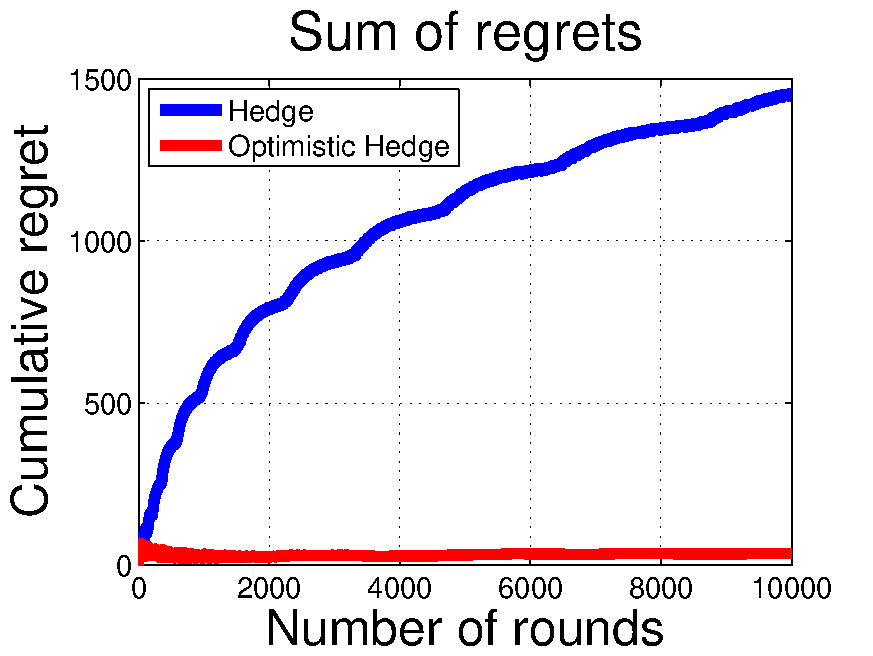
\includegraphics[width=0.4\textwidth,height=0.3\textwidth]{sum_regret.pdf}
}
\quad
\subfigure{
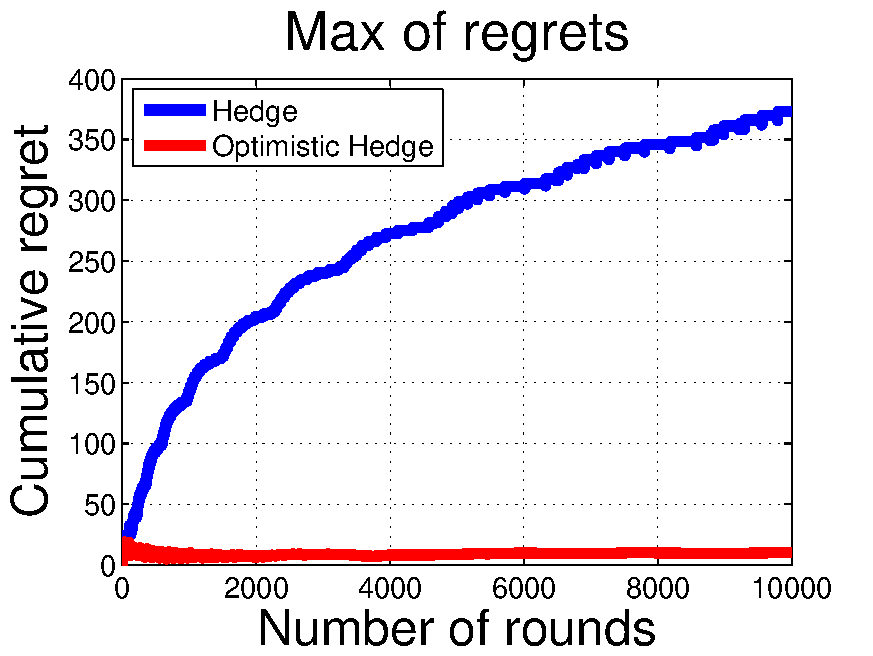
\includegraphics[width=0.4\textwidth,height=0.3\textwidth]{max_regret.pdf}
}
\caption{Maximum and sum of individual regrets over time under the
  Hedge (blue) and \mbox{Optimistic Hedge} (red) dynamics.}\label{fig:regrets}
\end{figure}



\begin{figure}[htbp]
\centering
\subfigure{
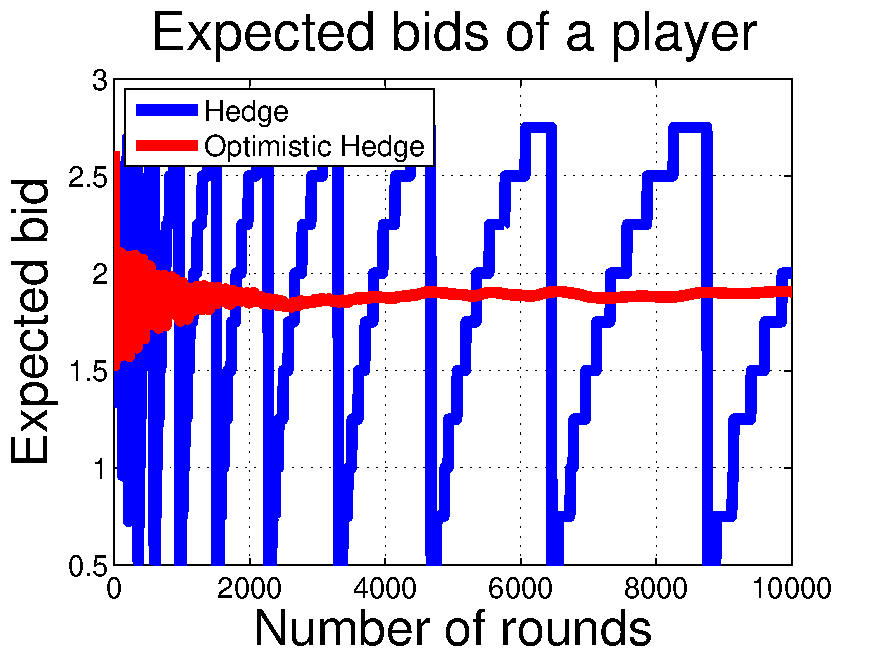
\includegraphics[width=0.4\textwidth,height=0.3\textwidth]{expected_bid.pdf}
}
\quad
\subfigure{
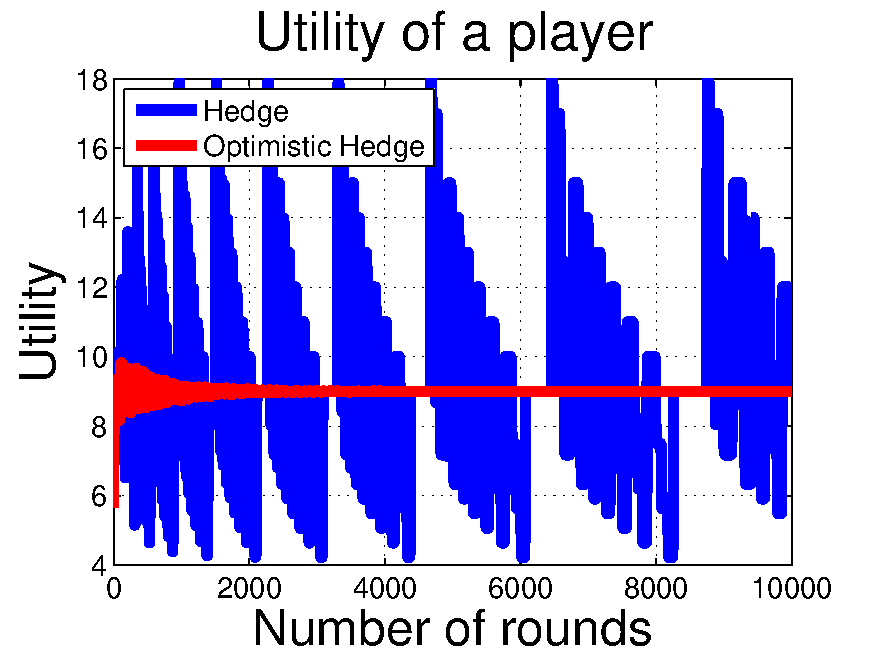
\includegraphics[width=0.4\textwidth,height=0.3\textwidth]{utilities.pdf}
}
\caption{Expected bid and per-iteration utility of a player on one of
  the four items over time, under Hedge (blue) and {Optimistic Hedge}
  (red) dynamics.}\label{fig:bids}
\end{figure}
\clearpage
\phantomsection

\addcontentsline{toc}{section}{Literatur}

%\thispagestyle{myheadings}
%\markright{Malte Schledjewski\hfill Elliptische Kurven und Beispielanwendungen in der Kryptologie\hfill}
\printbibliography


\end{document}
%%% Local Variables:
%%% mode: latex
%%% TeX-master: t
%%% End: